\section{Resultados}

Nesta seção, são apresentadas comparações entre as três políticas de navegação descritas anteriormente: passiva, \textit{greed} e \textit{simulated annealing}. O VANT percorre uma trajetória sistemática sobre a área de interesse (AI), sendo redirecionado dinamicamente de acordo com a política adotada ao detectar novos alvos.

\subsection{Valores de Entrada}

Os valores constantes utilizados no modelo são:

\begin{itemize}
    \item Tamanho da AI: $300 \times 300$ milhas náuticas (MN)
    \item Velocidade do VANT: 300 nós (MN / hora)
    \item Alcance do radar (detecção): 50 MN
    \item Alcance da câmera (inspeção): 20 MN
    \item Autonomia: 2400 MN
\end{itemize}

Os parâmetros que variam nas simulações são:

\begin{itemize}
    \item Número de navios na AI: 10, 25, 50, 75, 100, 125, 150, 175, 200. Esse parâmetro controla a densidade de alvos na área de interesse.
    
    \item Distribuição espacial dos navios: uniformente aleatória. As posições dos navios são sorteadas aleatoriamente dentro dos limites da área.
\end{itemize}

Os parâmetros utilizados especificamente na política de \textit{Simulated Annealing} são:

\begin{itemize}
    \item Temperatura inicial $T_0$: 10.0
    \item Temperatura mínima $T_{\text{min}}$: $10^{-4}$
    \item Fator de resfriamento $\beta$: 0.90
    \item Número de perturbações por temperatura: 50
\end{itemize}

Para cada combinação de parâmetros, os experimentos são repetidos sobre 100 instâncias geradas aleatoriamente, o que totaliza $3 \times 9 \times 100 = 2700$ simulações. Os resultados são agregados por média e as métricas são apresentadas em valores absolutos (como distância percorrida e tempo de execução) ou normalizados em percentual (como proporção de navios detectados ou inspecionados), conforme apropriado para a análise.

\subsection{Distância percorrida}

A Figura~\ref{fig:distancia} apresenta a média da distância total percorrida pelo VANT ao longo da missão, conforme a política de navegação e a quantidade de navios. A política \textit{passiva} mantém trajetória constante, enquanto as políticas com replanejamento (\textit{greed} e \textit{Simulated Annealing}) aumentam progressivamente a distância total percorrida à medida que mais navios são introduzidos no cenário.

\begin{figure}[H]
    \centering
    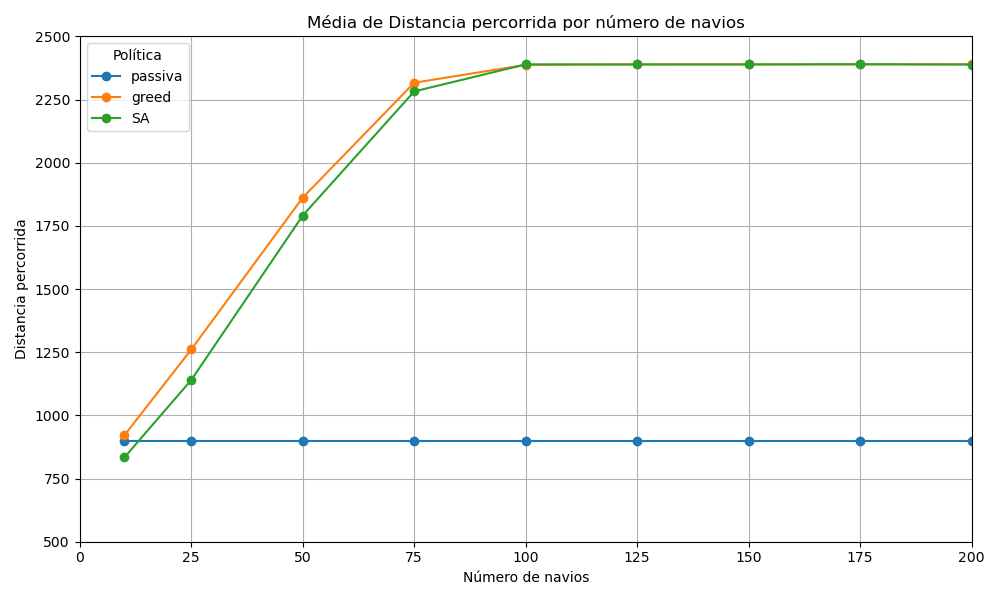
\includegraphics[width=0.7\textwidth]{fig/resultado_dis.png}
    \caption{Média da distância percorrida por política e quantidade de navios.}
    \label{fig:distancia}
\end{figure}

Observa-se que tanto a política \textit{greed} quanto a de \textit{Simulated Annealing} saturam a curva, atingindo a autonomia máxima do VANT a partir de 100 navios. Antes desse ponto de saturação, a política \textit{Simulated Annealing} percorre uma distância média menor do que a \textit{greed}, indicando que o método está encontrando soluções mais eficientes em termos de distância total percorrida.

\subsection{Detecção de navios}

A Figura~\ref{fig:detectados} mostra a média percentual de navios detectados ao longo da missão, considerando os que foram detectados ao menos uma vez, independentemente de terem sido inspecionados. A política \textit{passiva} apresenta uma taxa de detecção aproximadamente constante e significativamente mais alta do que as demais políticas, sendo inferior apenas em cenários entre 50 e 125 navios. Esse desempenho melhor faz sentido, pois, ao não se desviar da rota original, o VANT percorre toda a área de interesse, garantindo que todos os navios dentro do alcance do radar sejam detectados. 

\begin{figure}[H]
    \centering
    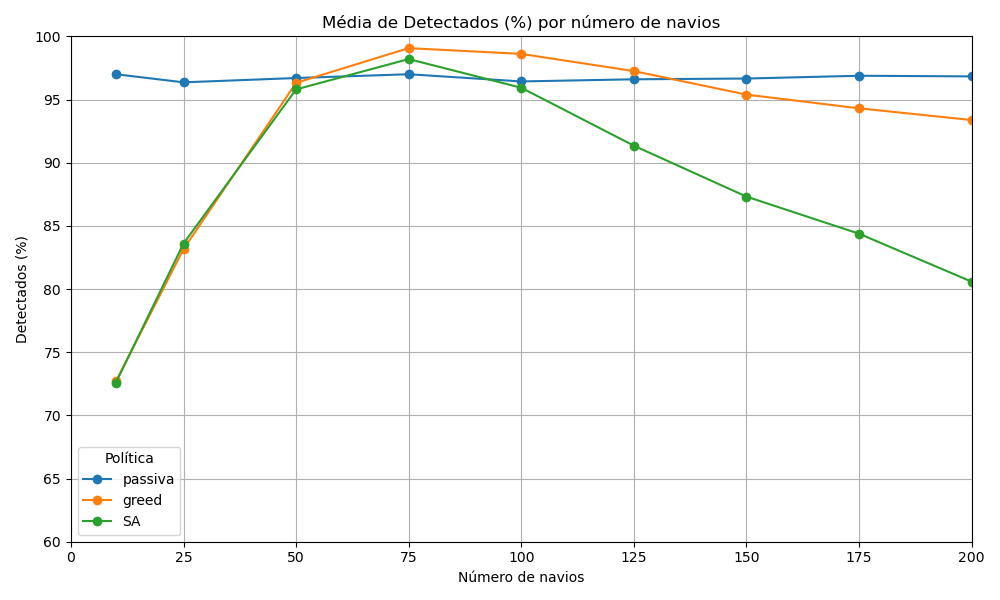
\includegraphics[width=0.7\textwidth]{fig/resultado_det.png}
    \caption{Média percentual de navios detectados por política e quantidade de navios.}
    \label{fig:detectados}
\end{figure}

As políticas \textit{greed} e \textit{Simulated Annealing}, por sua vez, apresentam desempenho próximo em cenários com até 75 navios, com diferenças mais evidentes a partir de cenários mais densos, onde o desempenho da política \textit{greed} tende a ser superior à política \textit{Simulated Annealing}. A taxa média de detecção tende a diminuir nas duas políticas, o que pode ser explicado pela figura \ref{fig:distancia}, que mostra que nesses cenários mais densos, o VANT atinge sua autonomia máxima, o que o obriga a interromper sua missão de inspeção.

\subsection{Inspeção de navios}

A Figura~\ref{fig:inspecionados} apresenta a média percentual de navios inspecionados em função da quantidade total de navios no cenário, para cada política de navegação considerada. Observa-se que a política\textit{passiva} mantem taxas de inspeção muito inferiores às políticas \textit{greed} e \textit{Simulated Annealing} em todos os cenários, o que é esperado, uma vez que estas duas políticas são projetadas para desviar da rota original, priorizando a inspeção de alvos relevantes ao longo da trajetória do VANT.

\begin{figure}[H]
    \centering
    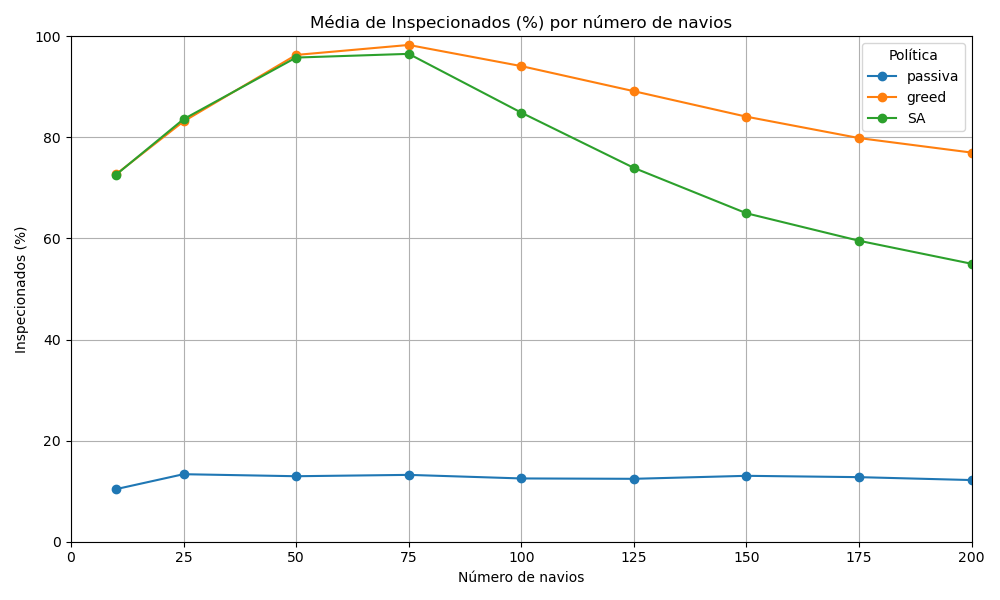
\includegraphics[width=0.7\textwidth]{fig/resultado_ins.png}
    \caption{Média percentual de navios inspecionados por política e quantidade de navios.}
    \label{fig:inspecionados}
\end{figure}

Assim como na detecção de navios, as políticas \textit{greed} e \textit{Simulated Annealing} apresentam desempenho próximo em cenários com até 75 navios, com diferenças mais evidentes a partir de cenários mais densos, onde o desempenho da política \textit{greed} tende a ser superior à política \textit{Simulated Annealing}. A taxa média de inspeção tende a diminuir nas duas políticas, o que pode ser explicado pela figura \ref{fig:distancia}, que mostra que nesses cenários mais densos, o VANT atinge sua autonomia máxima, o que o obriga a interromper sua missão de inspeção.

\subsection{Tempo de execução}

A Figura~\ref{fig:tempo_execucao} exibe o tempo médio de execução das simulações para cada política, em função do número de navios presentes no cenário. A política baseada em \textit{Simulated Annealing} apresenta tempo crescente conforme o número de navios aumenta, enquanto as políticas \textit{passiva} e \textit{greed} mantêm tempos iguais e praticamente constantes, muito inferiores aos da política \textit{Simulated Annealing}.

\begin{figure}[H]
    \centering
    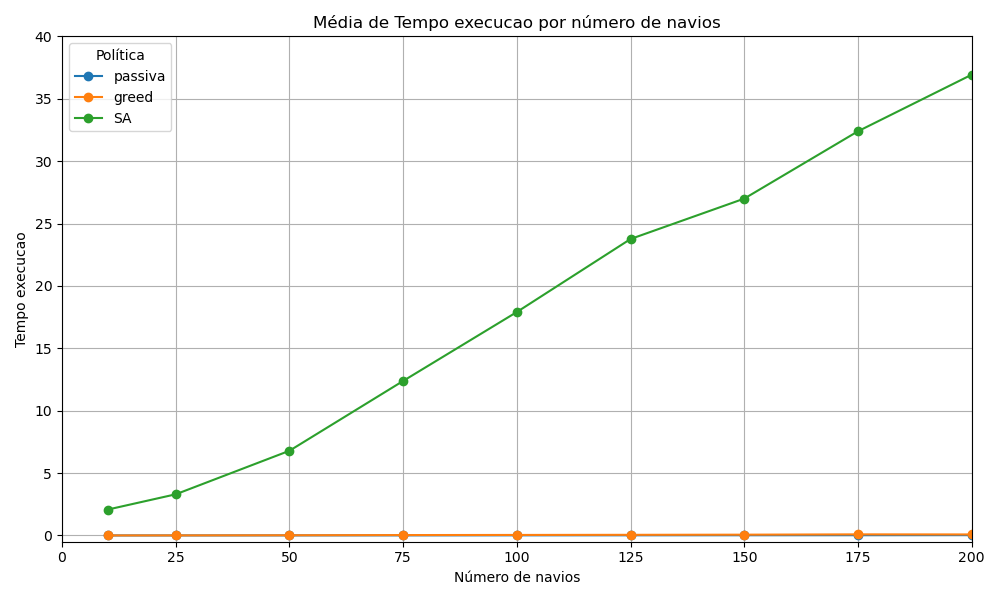
\includegraphics[width=0.7\textwidth]{fig/resultado_tem.png}
    \caption{Tempo médio de execução da simulação por política e quantidade de navios.}
    \label{fig:tempo_execucao}
\end{figure}

Apesar da quantidade de iterações dentro do algoritmo de \textit{Simulated Annealing}, depender apenas de $T_0$, $T_{\text{min}}$, $\beta$ e do número de perturbações para definir o número de iterações, a cada iteração é calculado o custo da rota, que é medido somando as distâncias entre dois pontos consecutivos. Uma vez que o número de pontos é a soma dos \textit{waypoints} ainda não alcançados e dos navios ainda não inspecionados, o que é executado em $O(n)$, onde $n$ é o número de pontos. Isso faz com que o tempo de execução cresça linearmente com o número de navios.

A política \textit{greed} também possui um custo computacional $O(n)$ para calcular a distância dos pontos em relaão ao vant e para ordenar eles. Porém esse valor não é múltiplicado pelo número de iterações, como ocorre no \textit{Simulated Annealing}, o que resulta em um tempo de execução constante e muito menor. 

\subsection{Comparação visual das trajetórias}

Esta subseção apresenta visualizações individuais da trajetória seguida pelo VANT em uma instância com 50 navios, utilizando as três políticas de navegação implementadas. Cada figura exibe a rota planejada (composta por waypoints paralelos), o caminho percorrido pelo VANT (trajetória real) e a localização dos navios inspecionados.

Na Figura~\ref{fig:trajetoria_passiva}, é mostrada a simulação utilizando a política \textit{passiva}. A Figura~\ref{fig:trajetoria_greed} exibe o cenário correspondente à política \textit{greed}, enquanto a Figura~\ref{fig:trajetoria_sa} mostra o resultado com a política baseada em \textit{Simulated Annealing}. As figuras destacam diferenças na forma como a trajetória é ajustada em tempo de voo e na distribuição espacial dos alvos inspecionados, de acordo com a política adotada.

\begin{figure}[H]
    \centering
    \begin{subfigure}{0.4\textwidth}
        \centering
        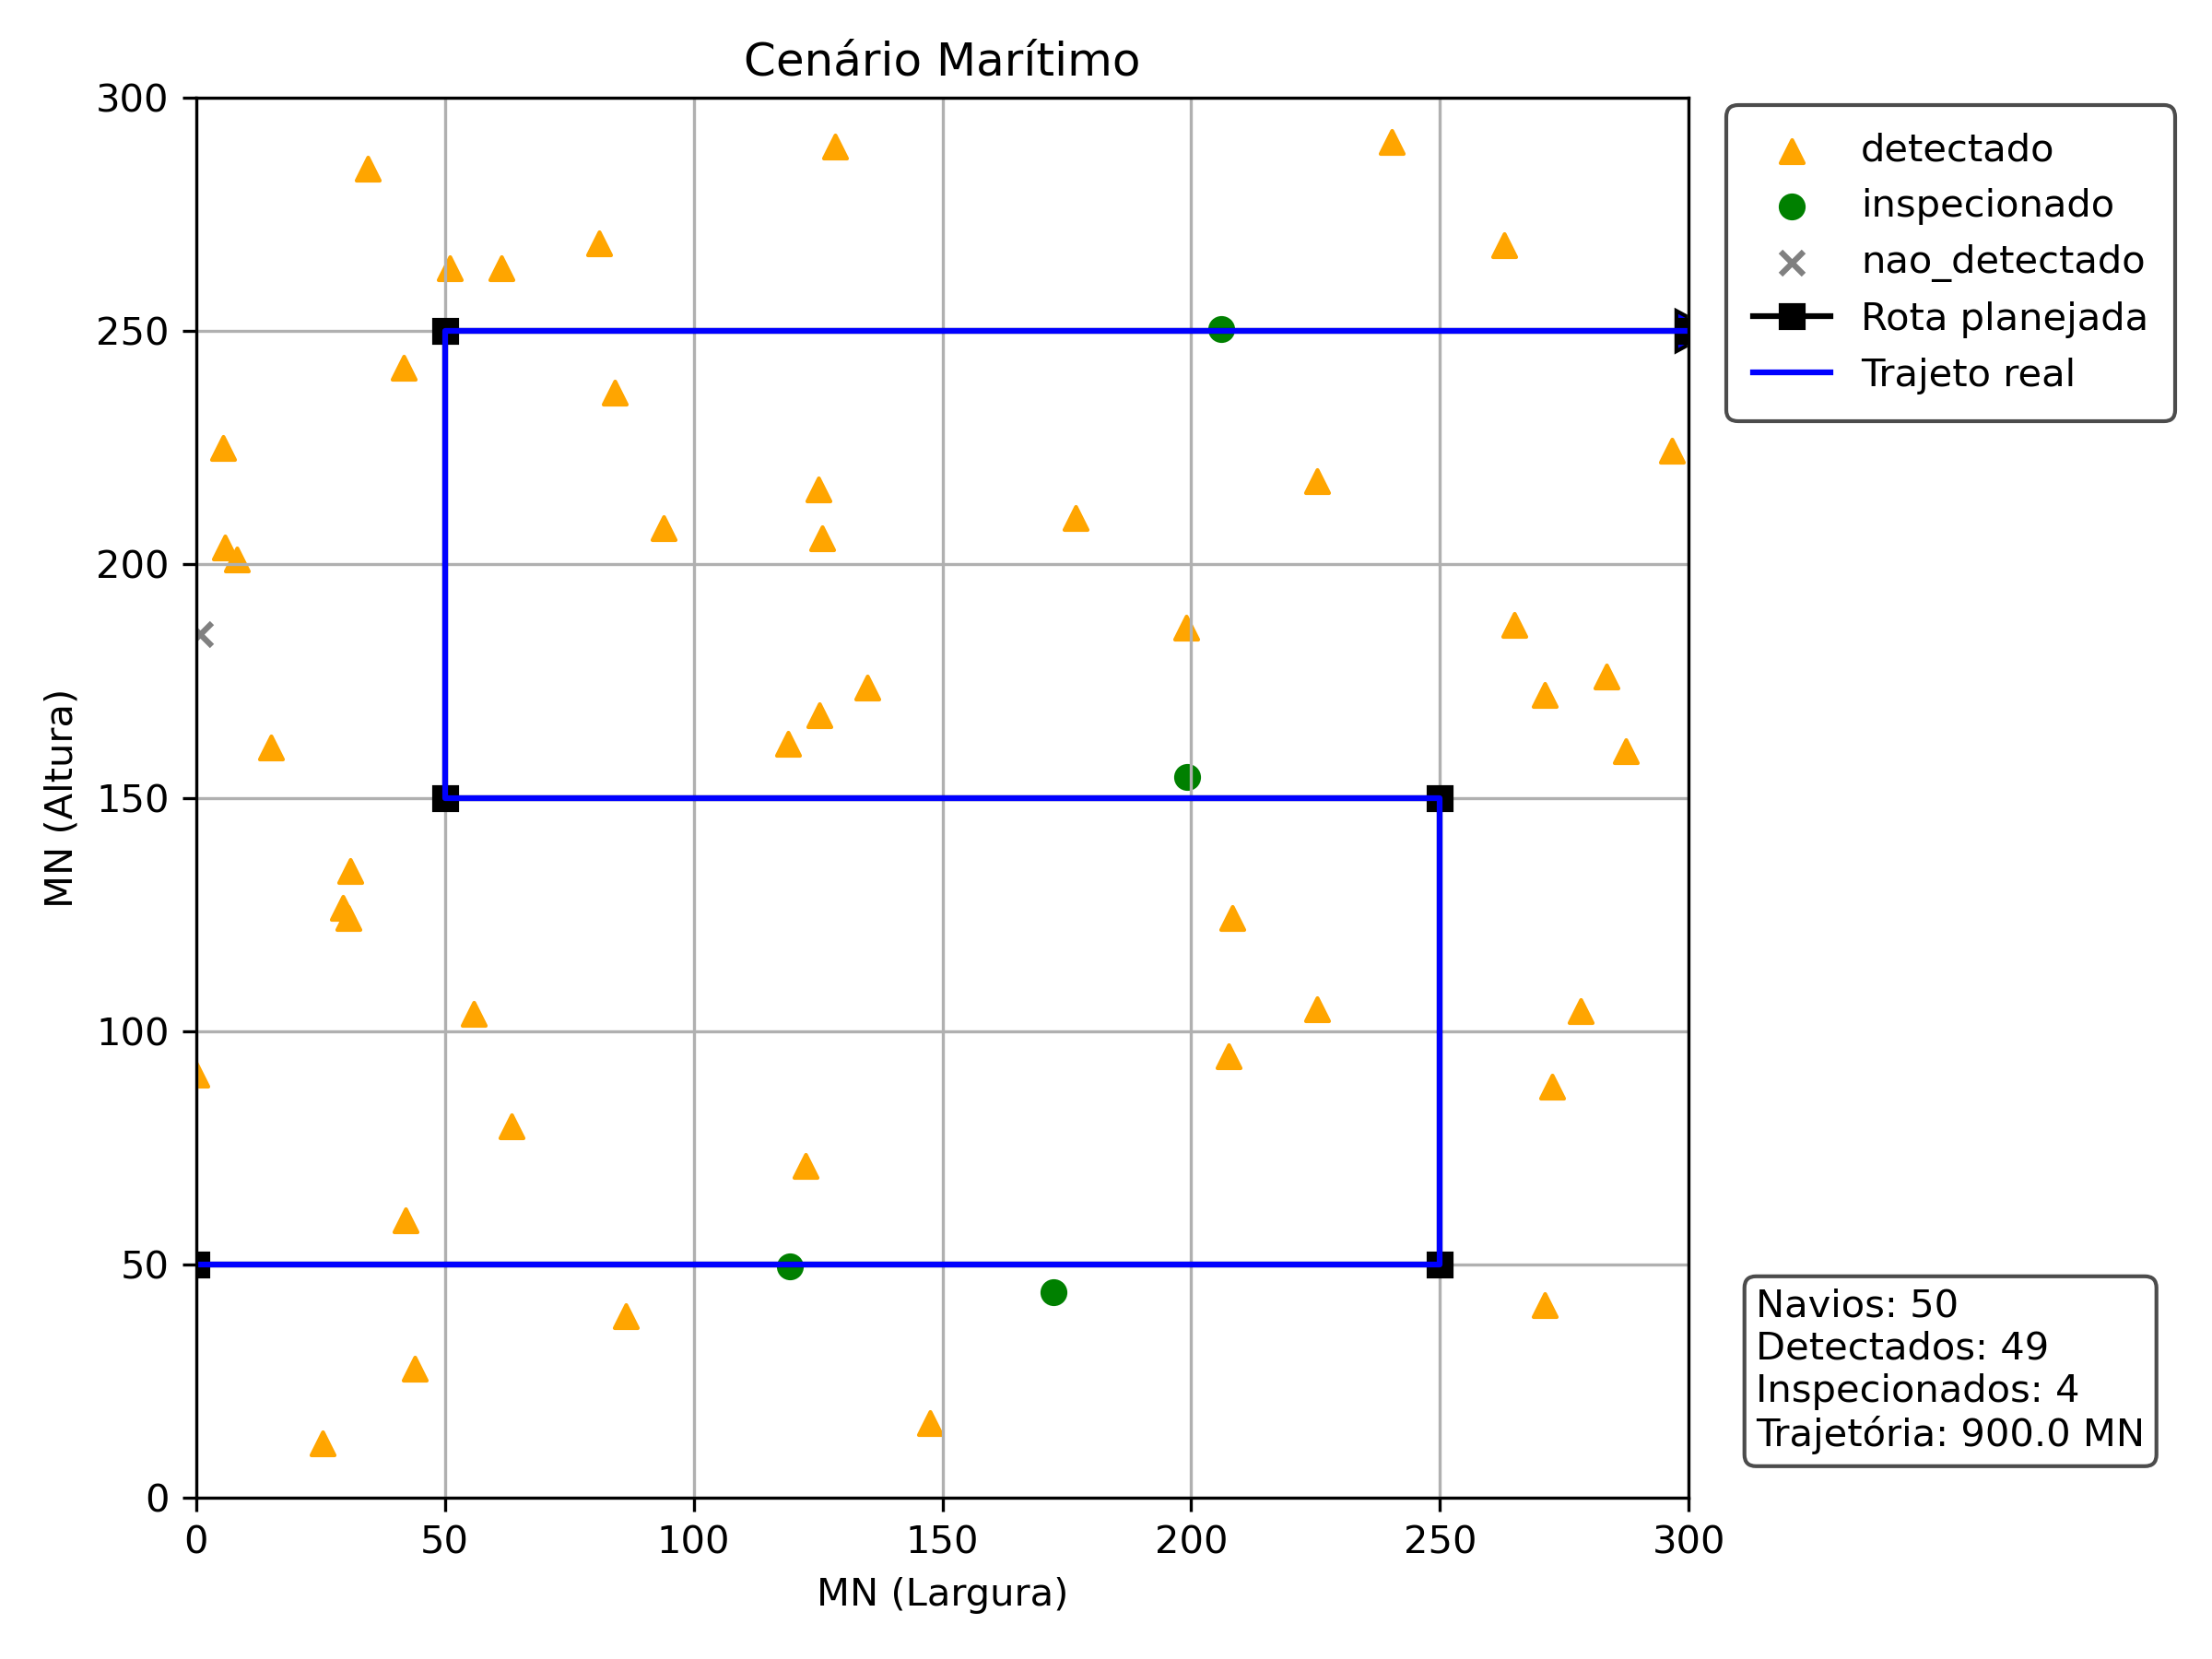
\includegraphics[width=\linewidth]{fig/passiva.png}
        \caption{\textit{Passiva}}
        \label{fig:trajetoria_passiva}
    \end{subfigure}
    \hfill
    \begin{subfigure}{0.4\textwidth}
        \centering
        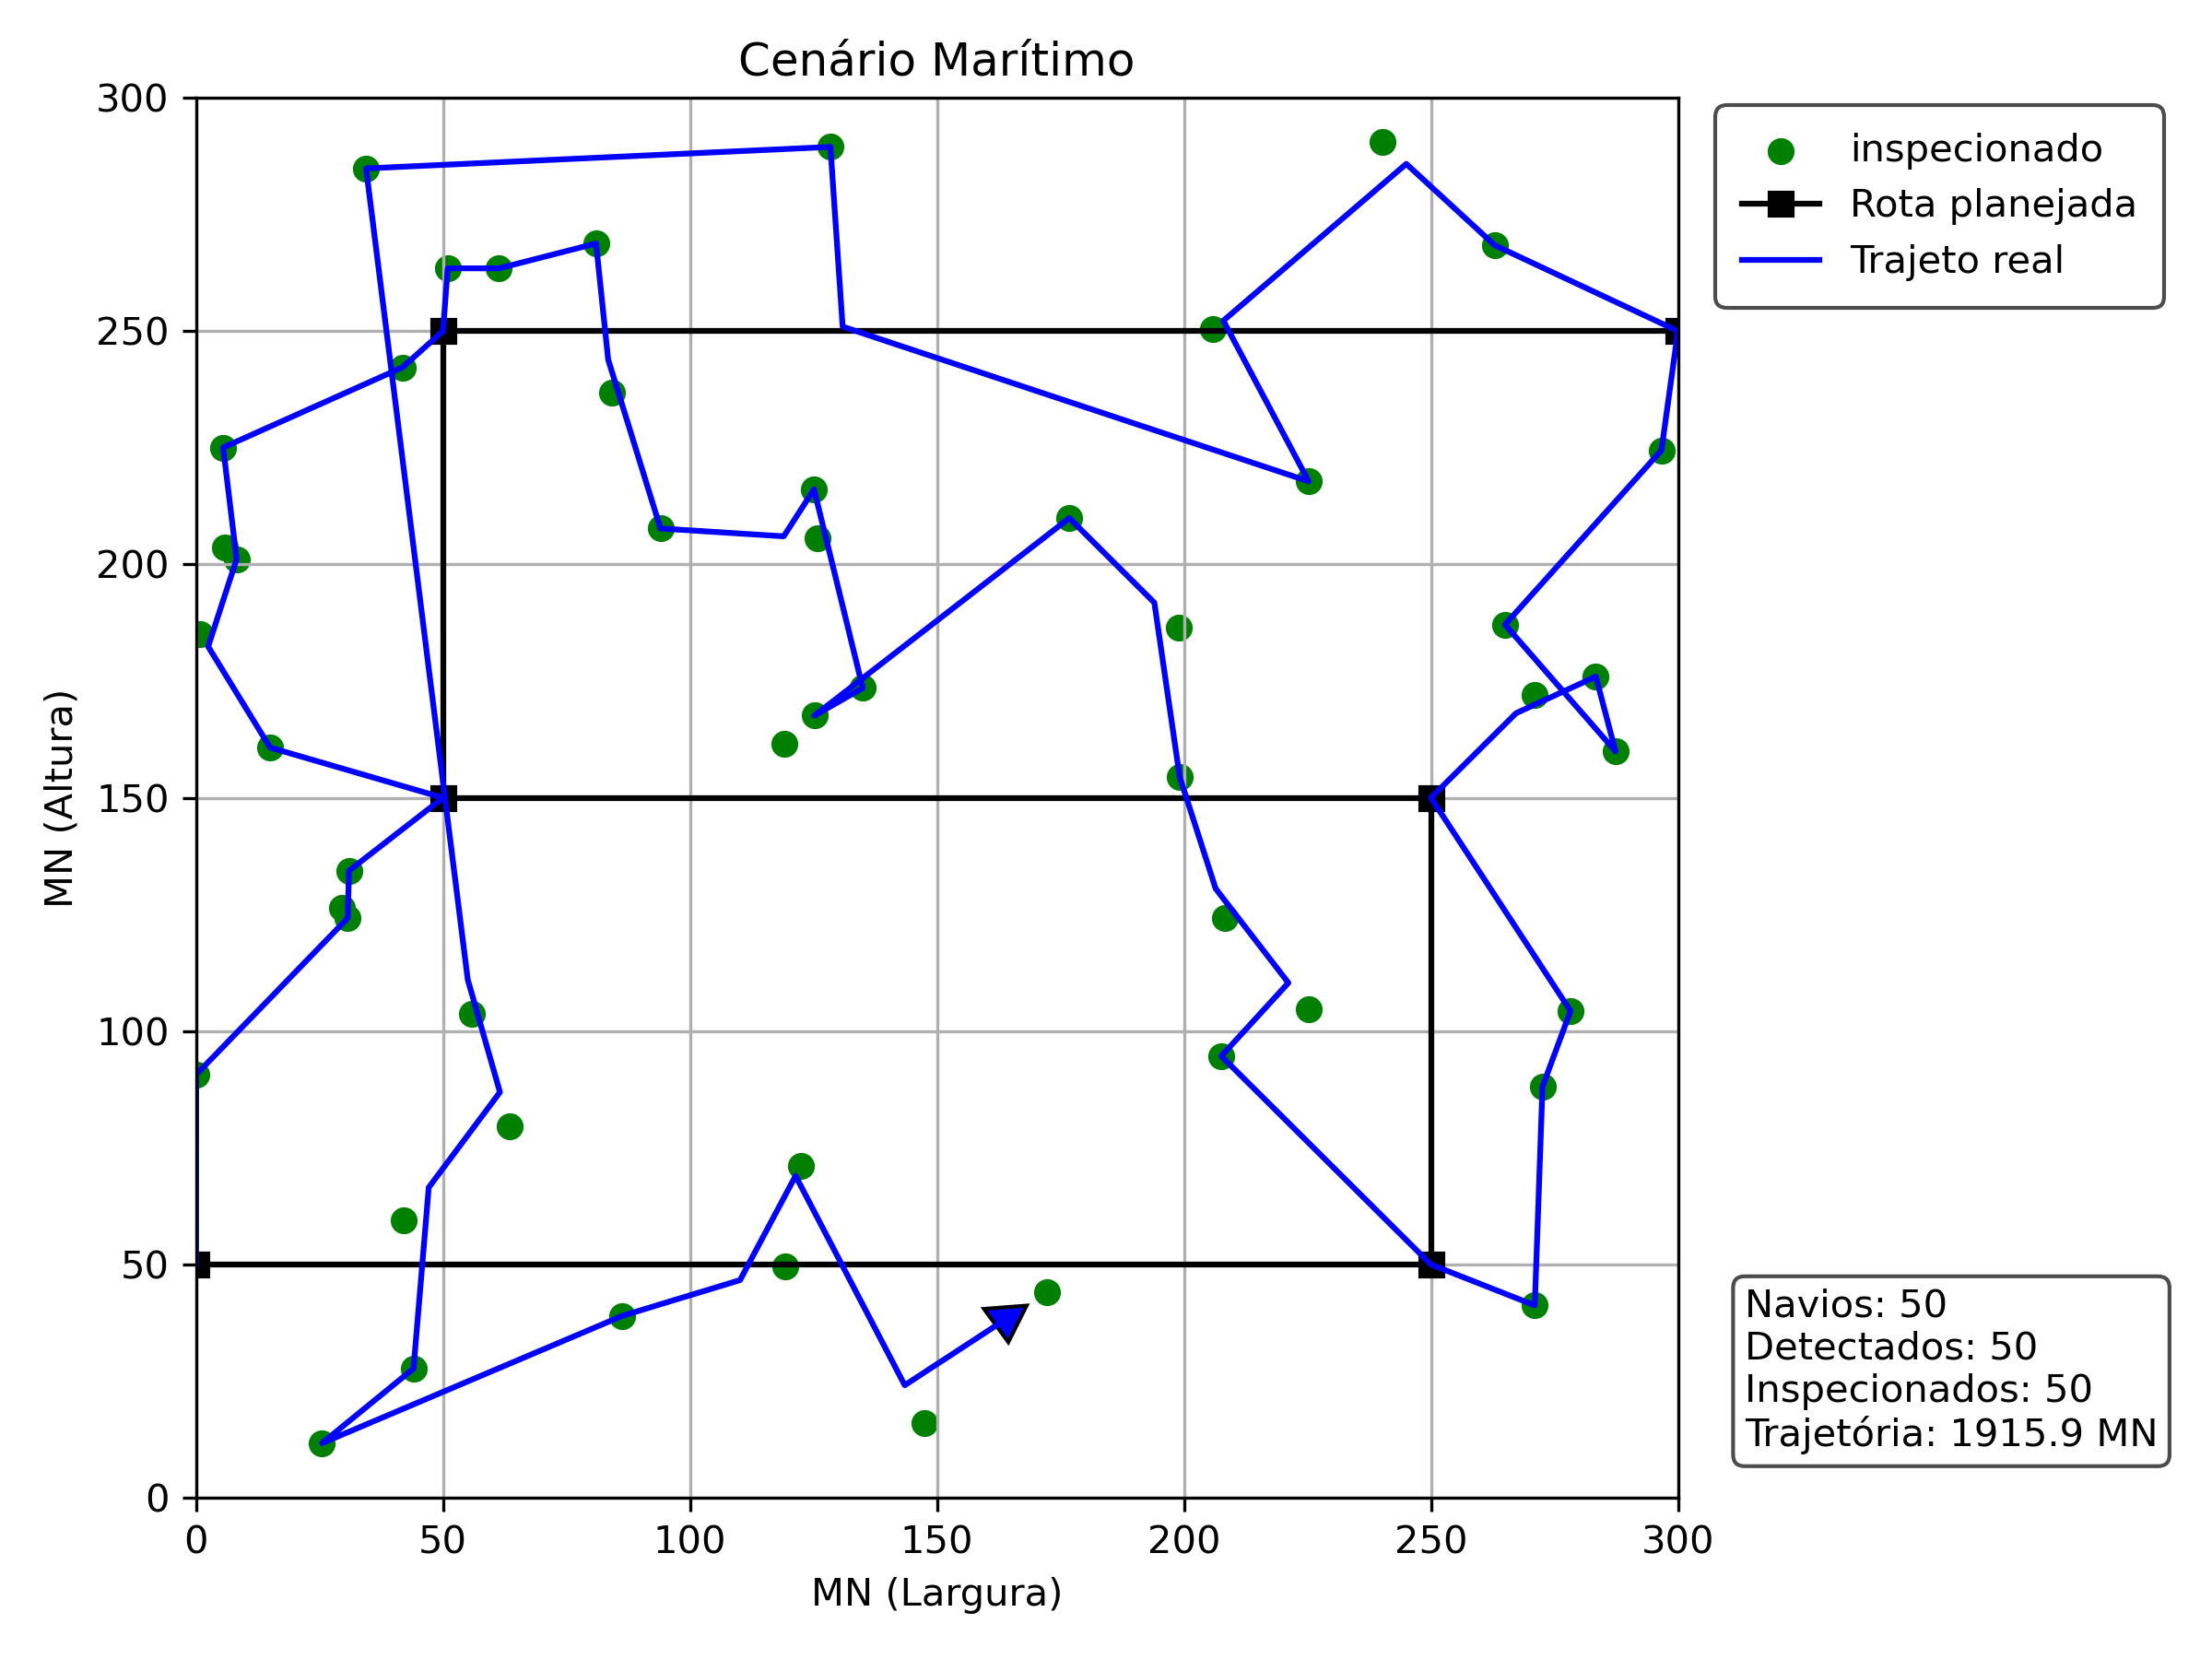
\includegraphics[width=\linewidth]{fig/greed.png}
        \caption{\textit{Greed}}
        \label{fig:trajetoria_greed}
    \end{subfigure}
    \hfill
    \begin{subfigure}{0.4\textwidth}
        \centering
        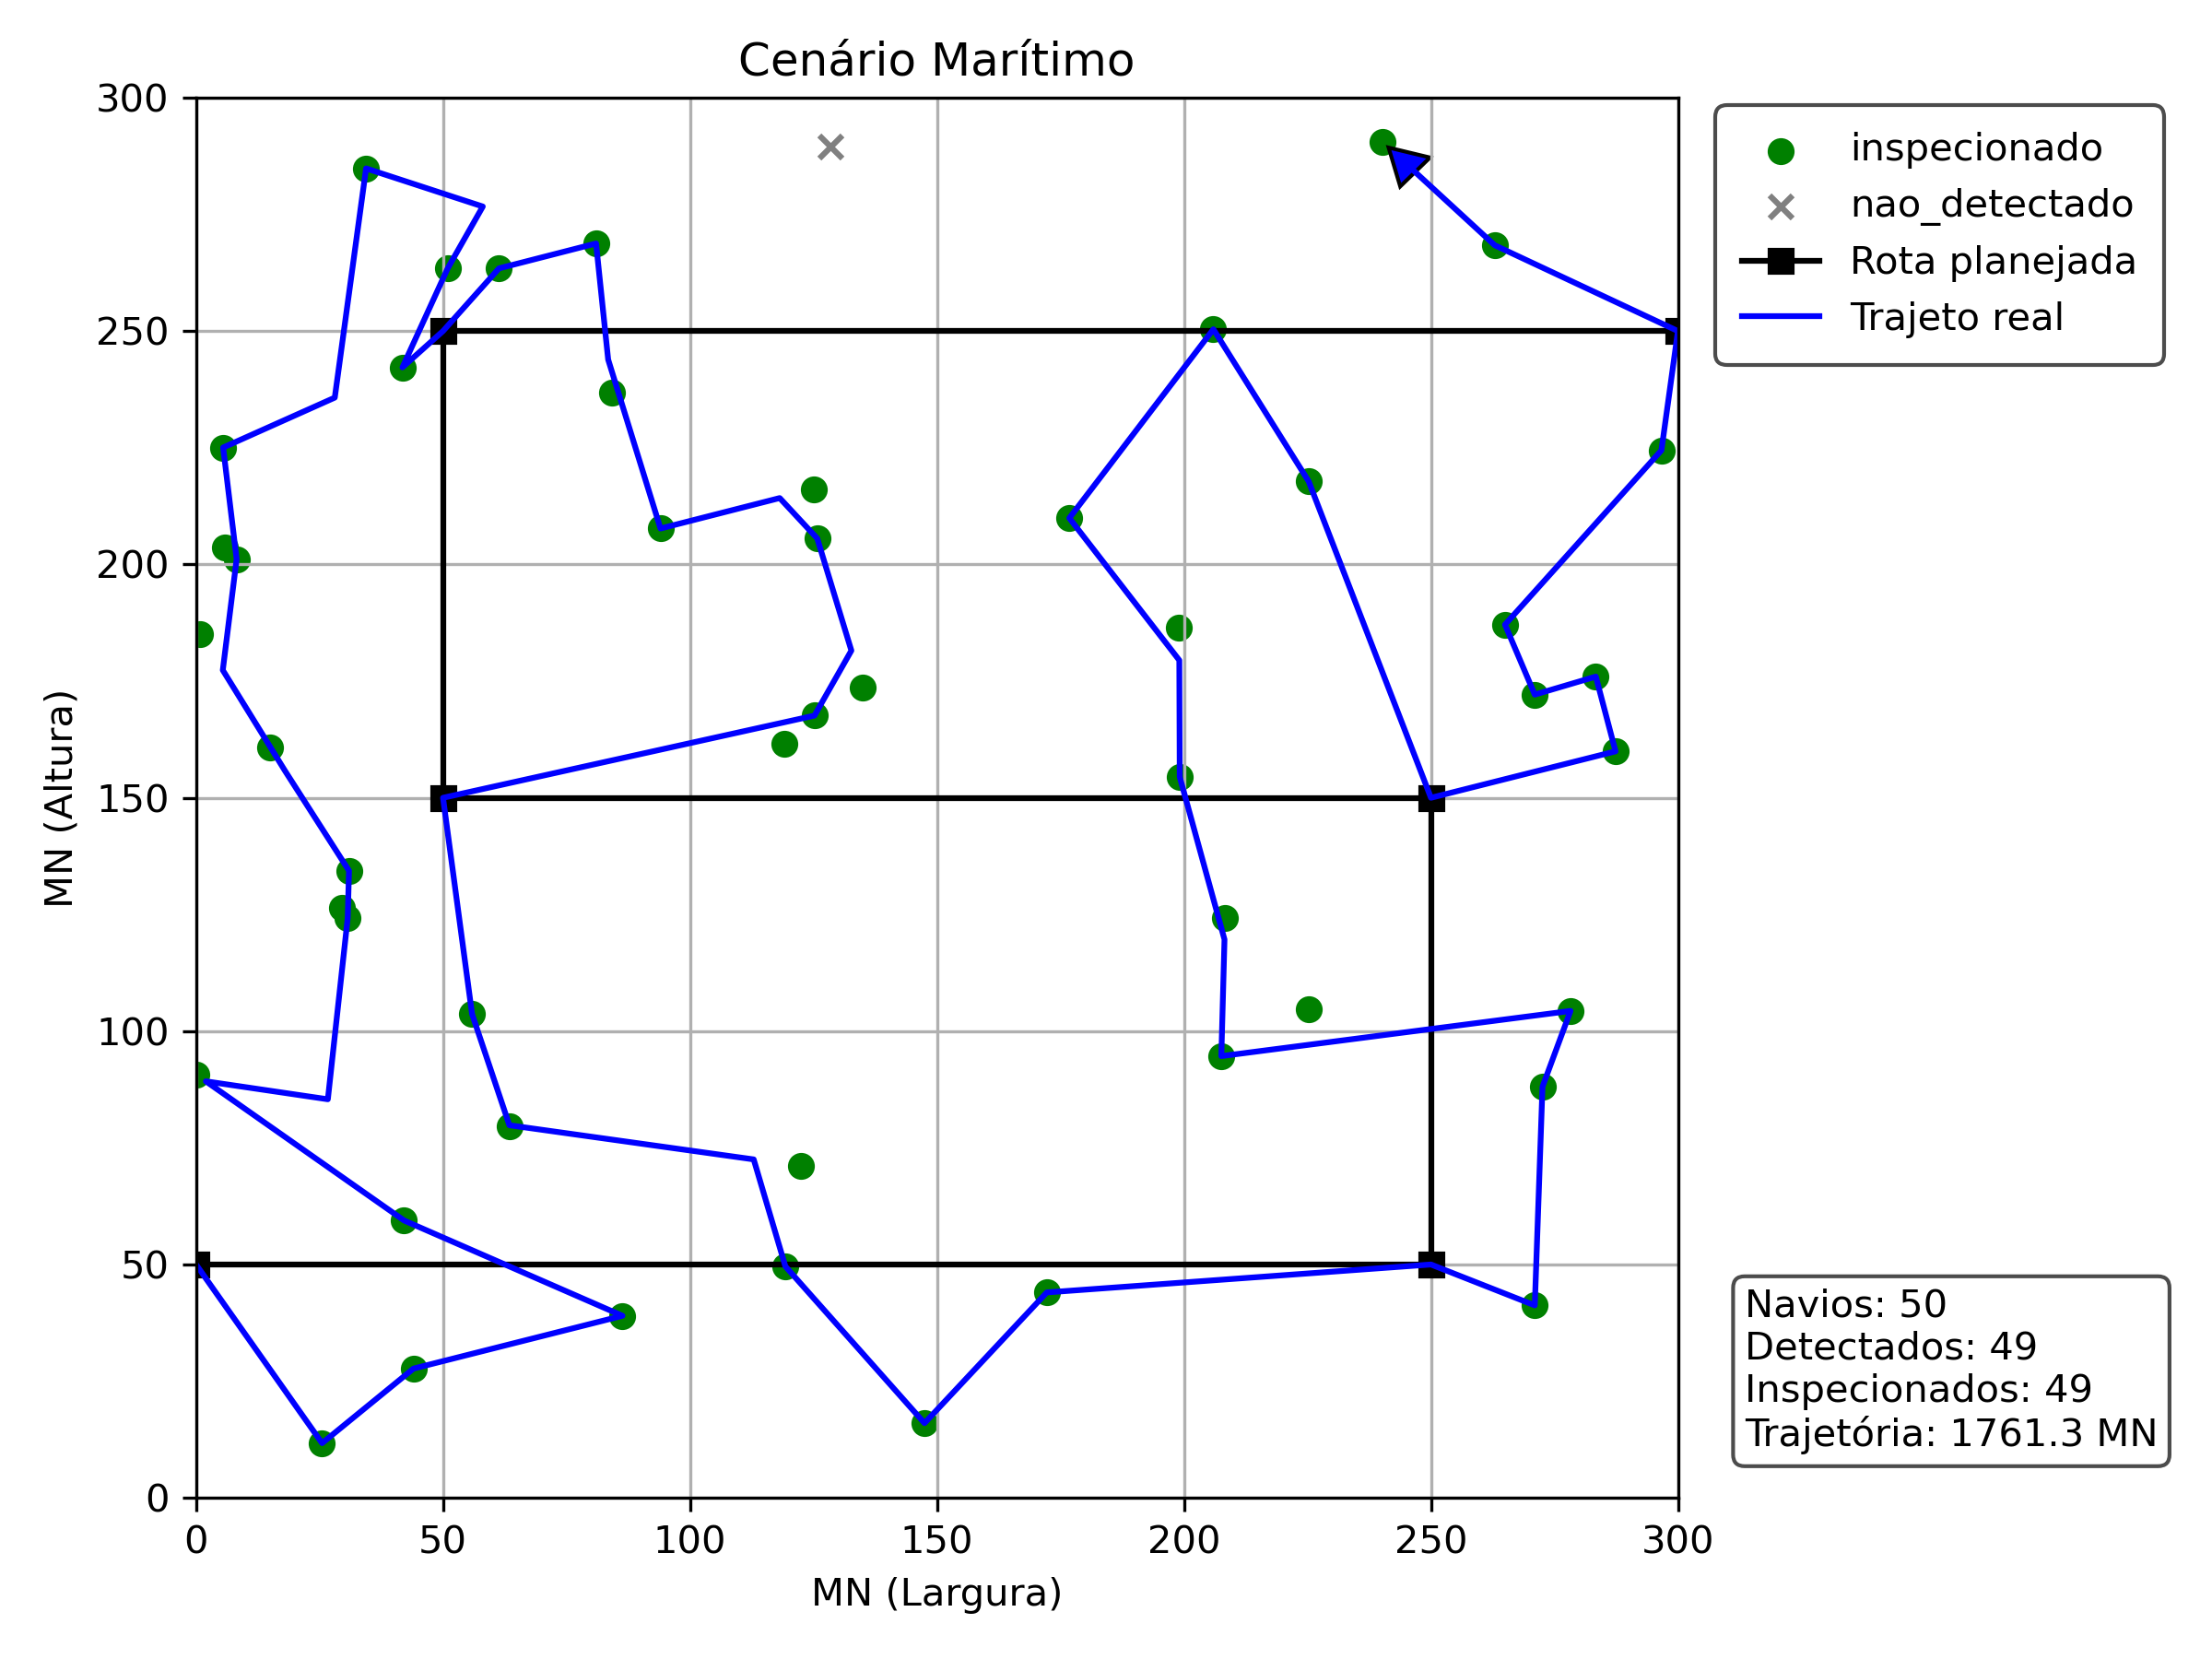
\includegraphics[width=\linewidth]{fig/SA.png}
        \caption{\textit{Simulated Annealing}}
        \label{fig:trajetoria_sa}
    \end{subfigure}
    \caption{Trajetória do VANT para as três políticas de navegação (50 navios).}
    \label{fig:trajetorias_comparacao}
\end{figure}

Na política \textit{passiva}, o VANT segue a rota de referência, inspecionando os navios que encontra ao longo do caminho. Já na política \textit{greed}, o VANT desvia da rota original para inspecionar os navios mais próximos, resultando em uma trajetória mais adaptativa. Por fim, na política \textit{Simulated Annealing}, o VANT também ajusta sua trajetória, mas de forma mais otimizada, buscando minimizar a distância total percorrida. Uma diferença notável é que, na política \textit{greed}, o VANT cruza a própria trajetória algumas vezes, o que não ocorre na política \textit{Simulated Annealing}. Isso indica que a política \textit{greed} pode ser menos eficiente em termos de distância total percorrida, pois revisita áreas já inspecionadas. Em contraste, a política \textit{Simulated Annealing} evita esse comportamento, resultando em uma trajetória mais direta e eficiente.


